\section{Human input}

By its nature, the problem is intrinsically unsupervised, for we do not know
before hand which place is similar to which one. Furthermore, there is no
easily available source containing this information at a large scale. The
traditional approach in recommendation system is to held off the most recent
data and compare the predicted result with them to assess its accuracy.  Yet
in this case, this method do not work. First because it restricts test users
to those that have spend a significant time in several cities. Second, even
among this limited pool, there would still not be enough information to
judge similarity. Consider someone who visited ten restaurants in Paris in
2010 and fifteen in London in 2012. We cannot infer from that that they are
all similar to each other, which mean we are still facing the original issue,
albeit at a smaller scale\footnote{A scale that potentially let us do manual
labeling though.}.

To overcome this difficulty of evaluating results, we decided to ask people
for their opinion. But as we thought it was to convoluted to ask directly for
pair of locations, we adopted a simpler approach. We presented user with a
list of activities (the full list is available in \autoref{tab:questions}) and
a map of a city. For each activity, user are prompted to draw region on the
map and optionally, select specific venues. The interface is showed in
\autoref{fig:survey}.

\begin{figure}[hbtp]
    \centering
    \begin{subfigure}[b]{\textwidth}
        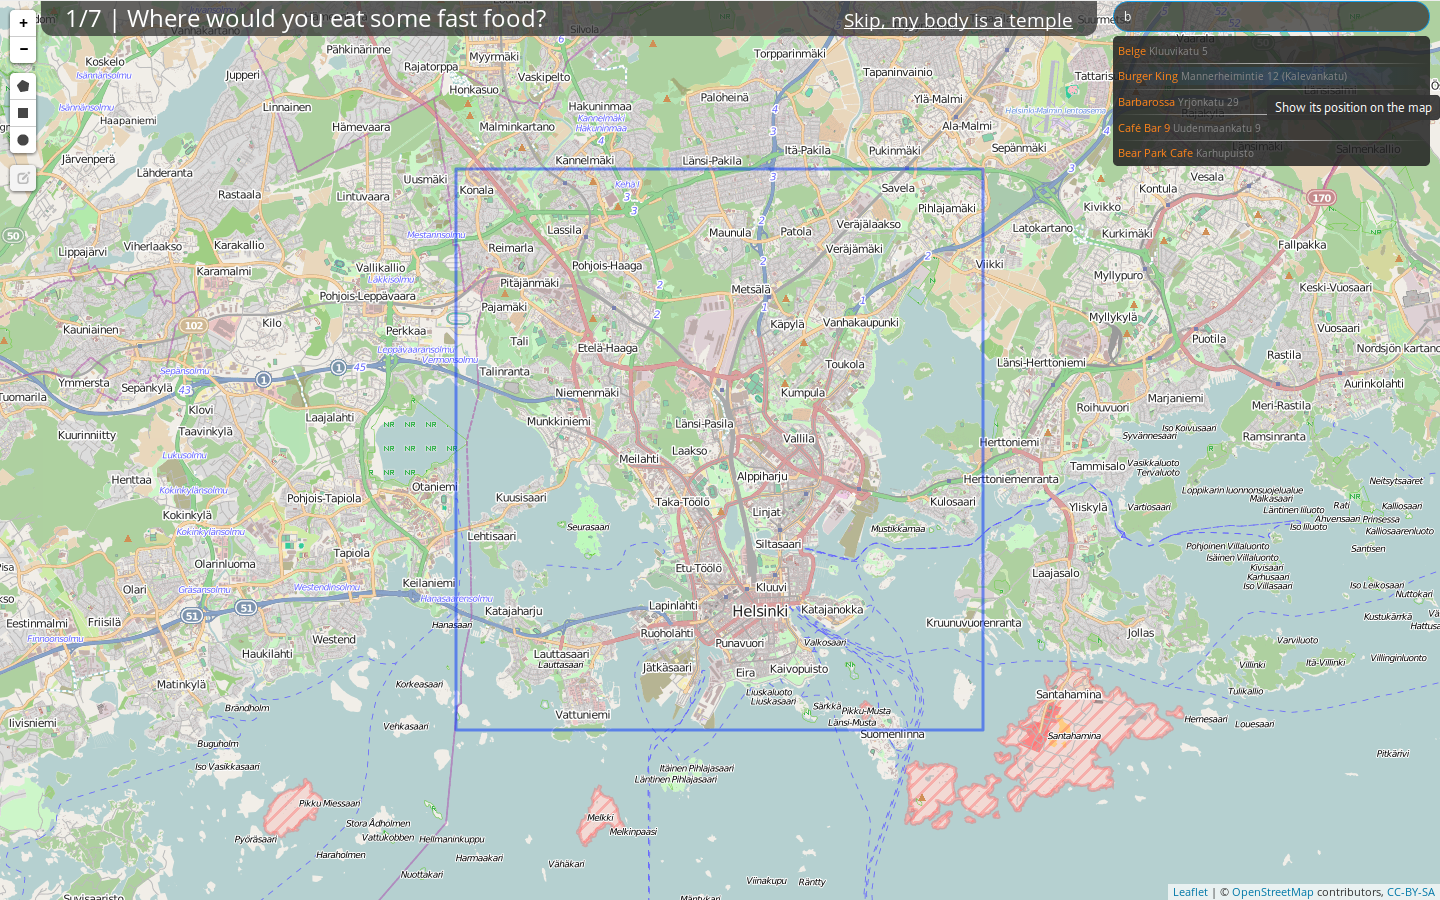
\includegraphics[width=\textwidth]{survey}
        \caption{The main screen of the survey.}
    \end{subfigure}

    \begin{subfigure}[b]{\textwidth}
        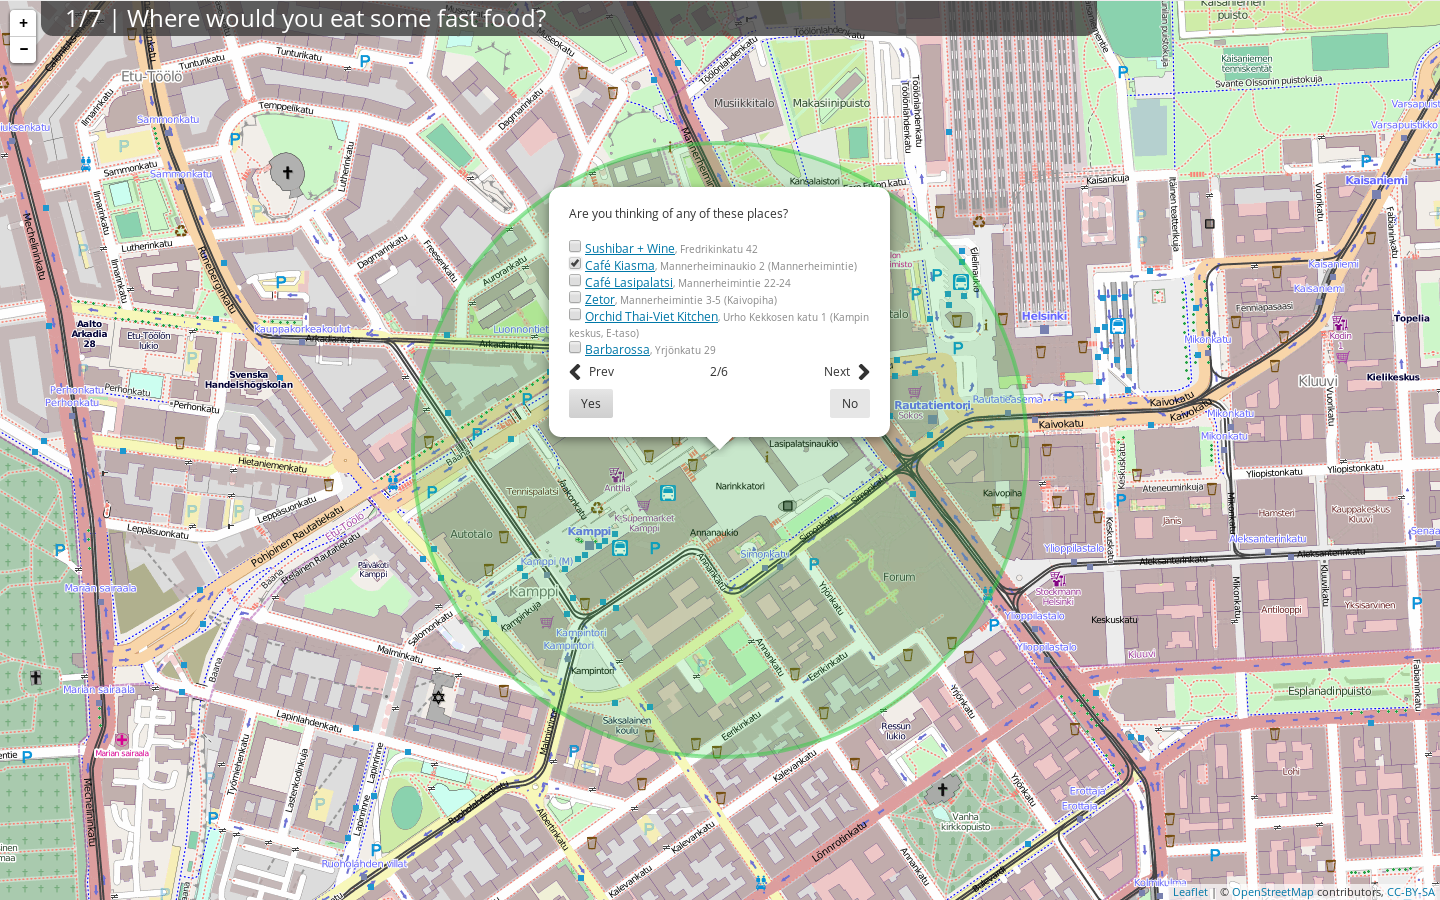
\includegraphics[width=\textwidth]{survey_venues}
        \caption{After an area have been drawn, the answer can be refined by
        choosing relevant venues from the dataset.}
    \end{subfigure}
    \caption{Website survey interface.\label{fig:survey}}
\end{figure}

\begin{comments}
number of answers, analysis of the results(?).
Rather tell about the slifht modification to ask directly for neighborhood
similar to those in Paris.
\end{comments}

\begin{table}[ht]
    \centering
    \begin{tabularx}{\textwidth}{lXX}
        \toprule
	Name & Question label & Relevant categories \\
        \midrule
	\texttt{fastfood} & Where would you eat some fast food?                       & Food \\
	\texttt{romance}  & Where would you bring your date to a romantic restaurant? & Food \\
	\texttt{coffee}   & Where would you drink a cozy coffee?                      & Tea Room, Bistro, Café, Coffee Shop, Cafeteria \\
	\texttt{clothes}  & Where would you buy new fancy clothes?                    & Clothing Store, Department Store, Fabric Shop, Flea Market, Mall \\
	\texttt{party}    & Where would you hangout with your friends?                & Nightlife Spot \\
	\texttt{sport}    & Where would you go to run in nature?                      &  Outdoors \& Recreation \\
	\texttt{culture}  & Where would you enjoy some cultural attractions?          & Art Gallery, Comedy Club, Concert Hall, Country Dance Club, Historic Site, Museum, Movie Theater, Music Venue, Outdoor Sculpture, Performing Arts Venue, Public Art, Street Art \\
        \bottomrule
    \end{tabularx}
    \caption[Question list]{The seven questions asked to gather human
    input.\label{tab:questions}}
\end{table}
